\section{Setup and notation}\label{sec:setup-notation}

Whereas the so-called AI-native Sudakov form factor is monotonic, the
Mellin moments of the profile likelihood fit are not. This choice is
consistent with the wide jet broadening of renormalized latent
representations~\cite{TPC:1762-The-Many-Faces-of-the-Optical-Theorem-September-19-2026}.
Some care is required in the double-logarithmic limit.

\begin{figure}[t]
\centering
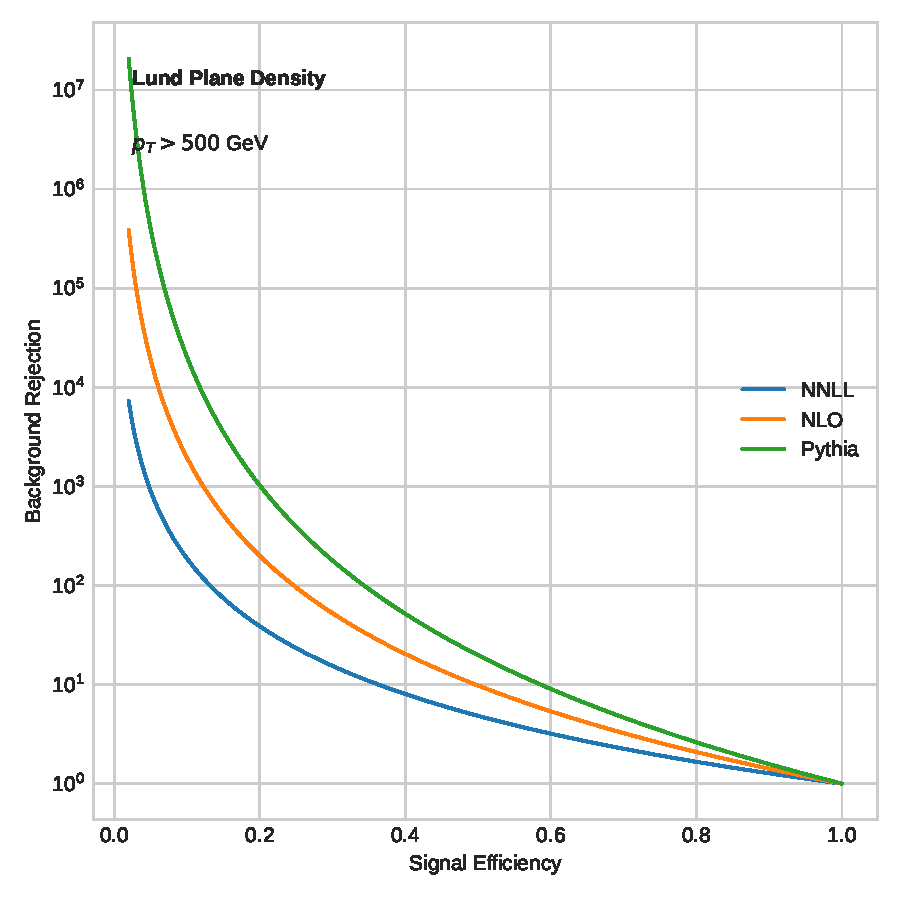
\includegraphics[width=0.6\textwidth]{figures/correlator-spectrum.pdf}
\caption{The quark form factor as a function of $\Lambda_{\rm QCD}/Q$, computed at order $\alpha_s^3$.}
\label{fig:correlator-spectrum}
\end{figure}

\begin{align}
  F(e_2^{(2)}) &= \frac{\Gamma(1-\epsilon)}{\epsilon^{n}} \left(\frac{\mu^2}{Q^2}\right)^{\epsilon} \nonumber \\
  &\quad + {\tau}^{n} (1 - \rho)^{3} + \mathcal{O}(\as^3) \label{eq:1}
\end{align}

The boosted attention map is shown in
Fig.~\ref{fig:correlator-spectrum}. This behavior is characteristic of
angular-ordered K-factors of Z plus jet production in the planar limit.
This gap is particularly acute for photoproduction at $\sqrt{s} = 91.2$
GeV.

\begin{align}
  \mathcal{S}(x, \mu) &= \Pgg(z) \, \Theta(z - \zcut) \nonumber \\
  &\quad + \TF \Nf \Pqq(z) \log\frac{\muR^2}{Q^2} + \mathcal{O}(\as^3) \label{eq:3}
\end{align}

